%%%% Paramétrage du TD %%%%
\def\xxactivite{\ifcolle Colle \else TD 2 \fi  \ifprof -- Corrigé \else \fi} % \normalsize \vspace{-.4cm}
\def\xxauteur{\textsl{Xavier Pessoles}}

%\def\xxnumchapitre{Chapitre 3 \vspace{.2cm}}
%\def\xxchapitre{\hspace{.12cm} Application du Principe Fondamental de la Dynamique}


\def\xxtitreexo{Stabilisateur passif d'image  \ifnormal $\star$ \else \fi \ifdifficile $\star\star$ \else \fi \iftdifficile $\star\star\star$ \else \fi }
\def\xxsourceexo{\hspace{.2cm} \footnotesize{Mines Ponts 2018 -- PSI}}


\def\xxcompetences{%
\vspace{.25cm}
\textsl{%
\textbf{Savoirs et compétences :***}
\begin{itemize}[label=\ding{112},font=\color{ocre}] 
%\item \textit{Mod2.C16} : torseur cinétique
%\item \textit{Mod2.C17} : torseur dynamique
\item \textit{Mod2.C17.SF1} : déterminer le torseur dynamique d’un solide, ou d’un ensemble de solides, par rapport à un autre solide
%\item \textit{Mod2.C15} : matrice d'inertie
\item \textit{Res1.C2} : principe fondamental de la dynamique
%\item \textit{Res1.C1.SF1} : proposer une démarche permettant la détermination de la loi de mouvement
%\item \textit{Res1.C2.SF1} : proposer une méthode permettant la détermination d’une inconnue de liaison
\end{itemize}
}}
\def\xxfigures{
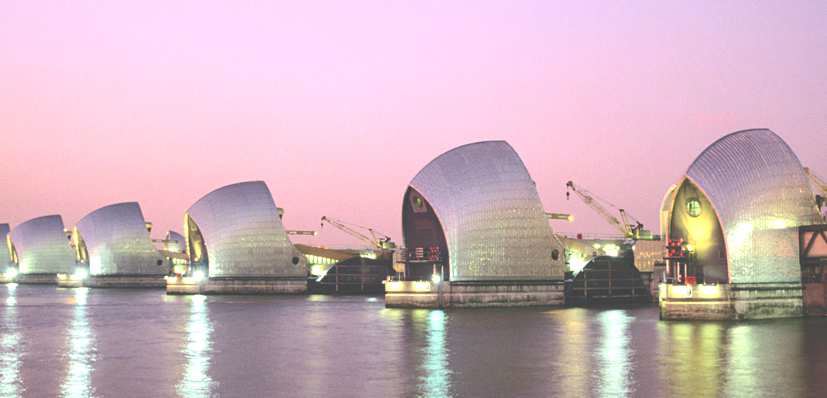
\includegraphics[width=.36\linewidth]{fig_00}
}%figues de la page de garde


\input{\repRel/Style/pagegarde_TD}
\setcounter{numques}{0}

\setlength{\columnseprule}{.1pt}

\pagestyle{fancy}
\thispagestyle{plain}

\ifprof
\vspace{4.8cm}
\else
\vspace{4.8cm}
\fi

\def\columnseprulecolor{\color{ocre}}
\setlength{\columnseprule}{0.4pt} 

%%%%%%%%%%%%%%%%%%%%%%%

\setcounter{exo}{0}




\ifprof
%\begin{multicols}{2}
\else
\begin{multicols}{2}
\fi

\subsection*{Mise en situation}
 \ifprof
 \else

Les appareils photos modernes fonctionnent en rafales : 8 à 10 images par seconde et en mode vidéo. Le besoin de
stabilisation de l’image dans de telles conditions est impératif. Le but de ce sujet est de s’intéresser au support de la caméra assurant la liaison entre le bras de l'utilisateur et la caméra elle-même.

Le stabilisateur se compose principalement de trois objets :
\begin{itemize}
\item une poignée orientable \textbf{(1)} manipulée directement par le photographe, liée au support \textbf{(2)} en $O$;
\item un support rigide \textbf{(2)} (\textbf{supposé sans masse}) sur lequel vient se fixer une caméra assimilée en première approximation à une masse ponctuelle $m_c$ placée en $G_c$ ;
\item un contrepoids lié à \textbf{(2)} et assimilé à une masse ponctuelle $m_{cp}$ placée en $G_{cp}$.
\end{itemize}

\begin{center}
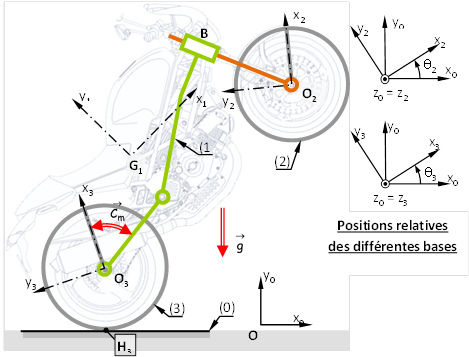
\includegraphics[width=.7\linewidth]{fig_01}
\end{center}

L’utilisateur tient fermement la poignée \textbf{(1)} dans une position angulaire quelconque, ce qui permet d’affirmer que le \textbf{(porteur + (1))} ne forme qu’une seule classe d’équivalence.
Afin de produire des images toujours fluides, sans à-coups, ce
stabilisateur à main doit maintenir constamment la caméra dans
une position verticale (parallèle au champ de
gravité), que le porteur soit immobile (plan fixe) ou en
mouvement (travelling).

Dans le cas général, le mouvement du bras par rapport au référentiel terrestre est quelconque (6 degrés de libertés). Ici, on se limite à un mouvement de translation. Dans le cas général, afin que la caméra soit en position verticale, le support doit permettre 3 rotations dans la liaison avec \textbf{(porteur + (1))}. Ici on se limite à la stabilisation d'une seule rotation. 
 \fi
\begin{obj}
Suite à une sollicitation brève de \SI{0,5}{m.s^{-2}}, l'amplitude des oscillations de la caméra ne doit pas dépasser les 0,5\degres.
\end{obj}

\subsection*{Travail demandé}
\ifprof
\else
On se place à présent dans une phase dite « dynamique ». Le porteur \textbf{(1)} est en mouvement par rapport au sol. On suppose qu'à l'instant initial, l'ensemble \textbf{(E)=Support(2) + Caméra(C) + Contrepoids(Cp)} est en équilibre stable en position verticale. On note $\torseurcin{V}{1}{0}=\torseurl{\vect{0}}{\vectv{P}{1}{0}=v(t)\vect{X_0}}{\forall P}$.
On note $a(t)=\dfrac{\dd v(t)}{\dd t}$. De plus, $\vect{OG_C}=L_C\vect{Z_2}$ et $\vect{OG_{CP}}=-L_{CP}\vect{Z_2}$.
\fi

\question{Par une étude dynamique que vous mettrez en \oe{}uvre, montrer que l'équation de mouvement de (E)
dans \textbf{(0)} galiléen s'exprime comme $Q_1\dfrac{\dd^2\varphi(t) }{\dd t^2}+Q_2(t)=Q_3(t)a(t)$.}

\ifdifficile
\ifprof
\else
\textit{Indication : vous commencerez par exprimer le bilan des actions mécaniques extérieures s’exerçant sur (E). Puis,
le théorème de la dynamique utilisé sera clairement énoncé. Enfin, les expressions des $Q_i$ en fonction de $m_c$,
$m_{cp}$, $L_c$, $L_{cp}$, $g$, $\sin\left(\varphi(t)\right)$ et $\cos\left(\varphi(t)\right)$ seront établies.}
\fi

\else
\fi


\ifprof
\begin{corrige}
\textbf{(1)} et \textbf{(E)} sont en liaison pivot d'axe $\axe{O}{Y_0}$. On va donc réaliser un théorème du moment dynamique appliqué à \textbf{(E)} en $O$ en projection sur $\vect{Y_0}$. 

\textbf{Calcul de $\vectmd{O}{E}{0}$}

\textbf{Méthode 1 -- En passant par le calcul de $\vectmd{O}{\text{2}}{0}$, $\vectmd{O}{\text{C}}{0}$ et $\vectmd{O}{\text{Cp}}{0}$}


Le support 2 étant sans masse, on a $\vectmd{O}{\text{2}}{0}=\vect{0}$. La caméra et le contrepoids étant considérés comme des masses ponctuelles, on a $\vectmd{G_C}{\text{C}}{0}=\vect{0}$ et $\vectmd{G_{Cp}}{\text{Cp}}{0}=\vect{0}$.

 \begin{tabular}{|p{.9\linewidth}}
\textbf{Calcul de $\vectmd{O}{\text{C}}{0}$}

 On a $\vectmd{O}{\text{C}}{0} = \vectmd{G_{C}}{\text{C}}{0}+\vect{OG_C} \wedge M_C\vectg{G_{C}}{\text{C}}{0}$.
 
\textbf{Calcul de $\vectg{G_{C}}{\text{C}}{0}$}

$\vectv{G_C}{\text{C}}{0}=\vectv{G_C}{\text{C}}{1}+\vectv{G_C}{\text{1}}{0}$ $=\vect{G_CO}\wedge \vecto{\text{C}}{0}+v(t)\vect{X_0}$ $=-L_C\vect{Z_2}\wedge \dot{\varphi}\vect{Y_2}+v(t)\vect{X_0}=L_C \dot{\varphi}\vect{X_2}+v(t)\vect{X_0}$.

De plus  $\vectg{G_C}{\text{C}}{0}=L_C \ddot{\varphi}\vect{X_2}-L_C \dot{\varphi}^2\vect{Z_2}+a(t)\vect{X_0}$.

Au final, $\vectmd{O}{\text{C}}{0} = \vect{OG_C} \wedge M_C\vectg{G_{C}}{\text{C}}{0}$
$ =L_C\vect{Z_2} \wedge M_C \left( L_C \ddot{\varphi}\vect{X_2}-L_C \dot{\varphi}^2\vect{Z_2}+a(t)\vect{X_0} \right)$

$\vectmd{O}{\text{C}}{0} =L_C M_C \left( L_C \ddot{\varphi}\vect{Y_2} +a(t) \cos \varphi \vect{Y_0} \right)$.

\end{tabular}

\vspace{.25cm}

 \begin{tabular}{|p{.9\linewidth}}
\textbf{Calcul de $\vectmd{O}{\text{Cp}}{0}$}

 On a $\vectmd{O}{\text{Cp}}{0} = \vectmd{G_{Cp}}{\text{Cp}}{0}+\vect{OG_{Cp}} \wedge M_{Cp}\vectg{G_{Cp}}{\text{C}}{0}$.

\textbf{Calcul de $\vectg{G_{Cp}}{\text{Cp}}{0}$}

De même, $\vectv{G_{Cp}}{\text{Cp}}{0}=\vectv{G_{Cp}}{\text{Cp}}{1}+\vectv{G_{Cp}}{\text{1}}{0}$ $=\vect{G_{Cp}O}\wedge \vecto{\text{Cp}}{0}+v(t)\vect{X_0}$ $=L_{Cp}\vect{Z_2}\wedge \dot{\varphi}\vect{Y_2}+v(t)\vect{X_0}=-L_{Cp} \dot{\varphi}\vect{X_2}+v(t)\vect{X_0}$. 

De plus  $\vectg{G_{Cp}}{\text{Cp}}{0}=-L_{Cp} \ddot{\varphi}\vect{X_2}+L_{Cp} \dot{\varphi}^2\vect{Z_2}+a(t)\vect{X_0}$. 

Au final, $\vectmd{O}{\text{Cp}}{0} = \vect{OG_{Cp}} \wedge M_{Cp}\vectg{G_{Cp}}{\text{Cp}}{0}$
$ =-L_{Cp}\vect{Z_2} \wedge M_{Cp} \left( -L_{Cp} \ddot{\varphi}\vect{X_2}+L_{Cp} \dot{\varphi}^2\vect{Z_2}+a(t)\vect{X_0}\right)$

$\vectmd{O}{\text{C}}{0} =-L_{Cp} M_{Cp} \left( -L_{Cp} \ddot{\varphi}\vect{Y_2} +a(t)\cos\varphi\vect{Y_0} \right)$
\\
\end{tabular}

On a donc $\vectmd{O}{E}{0}\cdot \vect{Y_0} =M_{Cp} L_{Cp}^2 \ddot{\varphi} -M_{Cp}L_{Cp}a(t)\cos\varphi +  M_CL_C^2 \ddot{\varphi} +M_CL_Ca(t) \cos \varphi $

\textbf{Méthode 2 -- En passant par le calcul de $\inertie{O}{E}$}

 \begin{tabular}{|p{.9\linewidth}}
On a $\inertie{O}{C}=M_C\matinertie{L_C^2}{L_C^2}{0}{0}{0}{0}{\mathcal{B}_2}$ et $\inertie{O}{Cp}=M_{Cp}\matinertie{L_{Cp}^2}{L_{Cp}^2}{0}{0}{0}{0}{\mathcal{B}_2}$ et donc 

$\inertie{O}{E}=\matinertie{M_{Cp}L_{Cp}^2+M_{C}L_{C}^2}{M_{Cp}L_{Cp}^2+M_{C}L_{C}^2}{0}{0}{0}{0}{\mathcal{B}_2}$.

$O$ est un point quelconque; donc $\vectmd{O}{E}{0}\cdot \vect{Y_0} =$

$\vectmd{O}{E}{R_0}=\left[\frac{\dd \vectmc{O}{E}{R_0}}{\dd t}\right]_{R_0}+\overrightarrow{V(O/R_0)}\wedge \overrightarrow{R_c}(E/R_0)$ et 
$\vectmc{O}{E}{R_0}=\inertie{O}{E}\cdot \vecto{E}{R_0}+M\;\vect{OG}\wedge \vectv{O}{E}{R_0}$. 

De plus, 
$\vect{OG}=\dfrac{M_CL_C-M_{Cp}L_{Cp}}{M_C+M_{Cp}}\vect{Z_2}$, $\vectv{O}{E}{R_0}=v(t)\vect{X_0}$ et
$\vectv{G}{E}{R_0}=v(t)\vect{X_0}+\dfrac{M_CL_C-M_{Cp}L_{Cp}}{M_C+M_{Cp}}\dot{\varphi}\vect{X_2}$.


On a donc, 
$\vectmc{O}{S}{R_0}=\dot{\varphi}\left(M_{Cp}L_{Cp}^2+M_{C}L_{C}^2 \right)\vect{Y_2}+\left( M_C+M_{Cp}\right) \dfrac{M_CL_C-M_{Cp}L_{Cp}}{M_C+M_{Cp}}\vect{Z_2}\wedge v(t)\vect{X_0}$
$ = \dot{\varphi}\left(M_{Cp}L_{Cp}^2+M_{C}L_{C}^2 \right)\vect{Y_2}+\left( M_CL_C-M_{Cp}L_{Cp}\right) v(t)\cos\varphi \vect{Y_0}$.

$\left[\frac{\dd \vectmc{O}{E}{R_0}}{\dd t}\right]_{R_0} =\ddot{\varphi}\left(M_{Cp}L_{Cp}^2+M_{C}L_{C}^2 \right)\vect{Y_2}+\left( M_CL_C-M_{Cp}L_{Cp}\right) \left( a(t)\cos\varphi - v(t)\dot{\varphi}\sin\varphi \right)\vect{Y_0}$.

$\overrightarrow{V(O/R_0)}\wedge \overrightarrow{R_c}(E/R_0) =v(t)\vect{X_0} \wedge \left(M_C+M_{Cp}\right) \left( v(t)\vect{X_0}+\dfrac{M_CL_C-M_{Cp}L_{Cp}}{M_C+M_{Cp}}\dot{\varphi}\vect{X_2} \right)$
$=\left(M_C+M_{Cp}\right) \left( \dfrac{M_CL_C-M_{Cp}L_{Cp}}{M_C+M_{Cp}}\dot{\varphi}v(t)\sin\varphi  \right)\vect{Y_2} $
$=\left( M_CL_C-M_{Cp}L_{Cp}  \right)\dot{\varphi}v(t)\sin\varphi\vect{Y_2} $.

Au final, $\vectmd{O}{E}{R_0}=\ddot{\varphi}\left(M_{Cp}L_{Cp}^2+M_{C}L_{C}^2 \right)\vect{Y_2}+\left( M_CL_C-M_{Cp}L_{Cp}\right)  a(t)\cos\varphi \vect{Y_0}$
\\

\end{tabular}

\textbf{Bilan des actions mécaniques en $O$ agissant sur $E$}
\begin{itemize}
\item Liaison pivot $\torseurstat{T}{1}{E}$ avec $\vectm{O}{1}{E}\cdot \vect{Y_2}=0$. 
\item $\torseurstat{T}{\text{pes}}{C}$ avec $\vectm{O}{\text{pes}}{C}\cdot \vect{Y_2}=\left( \vect{OG_C}\wedge -M_Cg \vect{Z_0}\right) \vect{Y_2}$ $=\left( L_C\vect{Z_2}\wedge -M_Cg \vect{Z_0}\right) \vect{Y_2}$
$= L_CM_Cg \sin \varphi  \vect{Y_2}$. 
\item $\torseurstat{T}{\text{pes}}{Cp}$ avec $\vectm{O}{\text{pes}}{Cp}\cdot \vect{Y_2}$%=\left( \vect{OG_{Cp}}\wedge -M_{Cp}g \vect{Z_0}\right) \vect{Y_2}$ 
$=\left( -L_{Cp}\vect{Z_2}\wedge -M_{Cp}g \vect{Z_0}\right) \vect{Y_2}$
$=- L_{Cp}M_{Cp}g \sin \varphi  \vect{Y_2}$. 
\end{itemize}

\textbf{Théorème du moment dynamique en $O$ en projection sur $\vect{Y_2}$}

$\ddot{\varphi}\left(M_{Cp}L_{Cp}^2+M_{C}L_{C}^2 \right)+\left( M_CL_C-M_{Cp}L_{Cp}\right)  a(t)\cos\varphi =
 L_CM_Cg \sin \varphi- L_{Cp}M_{Cp}g \sin \varphi $.

$\Leftrightarrow \ddot{\varphi}\left(M_{Cp}L_{Cp}^2+M_{C}L_{C}^2 \right)
+\left(   L_{Cp}M_{Cp} - L_CM_C \right)g \sin \varphi=
  - \left( M_CL_C-M_{Cp}L_{Cp}\right)  a(t)\cos\varphi $.

On a donc : 
$Q_1 = M_{Cp}L_{Cp}^2+M_{C}L_{C}^2 $, $Q_2(t)=\left(   L_{Cp}M_{Cp} - L_CM_C \right)g \sin \varphi$, 
$Q_3(t)= \left(M_{Cp}L_{Cp}- M_CL_C\right)  \cos\varphi$.
\end{corrige}
\else
\fi
 
 
\ifprof
\else
Afin de quantifier la modification d’attitude de (E), l'équation de mouvement est linéarisée autour de la position
d'équilibre (verticale) en supposant que les valeurs de l'angle restent faibles. On transpose cette équation
différentielle dans le domaine de Laplace et on note $\mathcal{L}\left(\varphi(t) \right)=\Phi(p)$ et $\mathcal{L}\left(a(t) \right)=A(p)$. 
Afin de conserver la fluidité des images lors de travelling, les fluctuations indésirables des mouvements du porteur ne
doivent pas être intégralement transmisses à (E).

On suppose que $a(t)=a_0\sin \left( \omega_a t\right)$ avec $a_0=\SI{0,5}{m.s^{-2}}$ et $g=\SI{10}{m.s^{-2}}$.
\fi

\question{Établir sous forme canonique la fonction de transfert $H(p)=\dfrac{\Phi(p)}{A(p)}$. Donner l'expression de la pulsation propre $\omega_0$ en fonction de $m_c$, $m_{cp}$, $L_{c}$, $L_{cp}$ et $g$.}
\ifprof
\begin{corrige}
Dans les conditions précédentes, on a $Q_1 = M_{Cp}L_{Cp}^2+M_{C}L_{C}^2 $, $Q_2(t)=\left(   L_{Cp}M_{Cp} - L_CM_C \right)g  \varphi$ et $Q_3(t)=  \left(M_{Cp}L_{Cp}- M_CL_C\right)$.

L'équation de comportement devient donc  $Q_1\dfrac{\dd^2\varphi(t) }{\dd t^2}+\left(   L_{Cp}M_{Cp} - L_CM_C \right)g  \varphi=Q_3a(t)$ 

$ \Rightarrow Q_1 p^2 \Phi(p) + \left(   L_{Cp}M_{Cp} - L_CM_C \right)g  \Phi(p)=Q_3A(p)$ et $H(p)=\dfrac{Q_3}{ Q_1 p^2  + \left(   L_{Cp}M_{Cp} - L_CM_C \right)g  }$.

On a donc $\omega_0^2 = \dfrac{\left(   L_{Cp}M_{Cp} - L_CM_C \right)g }{Q_1}=\dfrac{\left(   L_{Cp}M_{Cp} - L_CM_C \right)g }{ M_{Cp}L_{Cp}^2+M_{C}L_{C}^2}$. 
Le gain $K$ vaut $\dfrac{M_{Cp}L_{Cp}- M_CL_C}{\left(   L_{Cp}M_{Cp} - L_CM_C \right)g}=\dfrac{1}{g}$.
\end{corrige}
\else
\fi

\question{Tracer l'allure du diagramme asymptotique de gain $G_{\text{dB}}=f\left( \omega\right)$ de la fonction de transfert $H\left(j\omega\right)$. Placer les caractéristiques remarquables.}
\ifprof
\begin{corrige}~\\

\begin{center}
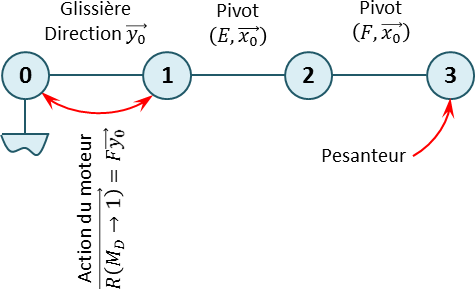
\includegraphics[width=.6\linewidth]{cor_01}
\end{center}
\end{corrige}
\else
\fi


\question{Pour un fonctionnement filtrant satisfaisant, on impose que $\omega_0=0,1\omega_a$. Le stabilisateur est réglé en
conséquence par l’intermédiaire du couple $\left( m_{cp},L_{cp}\right)$. En utilisant le comportement asymptotique en gain de $G_{\text{dB}}$, estimer numériquement l'amplitude $\Delta \varphi$ (en degrés) des oscillations de $\textbf{(E)}$
selon l'axe $\axe{O}{y_0}$.}
\ifprof
\begin{corrige}
On a $\omega_a=10\omega_0$. Une décade après $\omega_0$, $G_{\text{dB}}=-20\log 10 - 40 = \SI{-60}{dB}$. Une atténuation de \SI{-60}{dB} correspond à un gain de $10^{-\dfrac{60}{20}}=0,001$. L'amplitude des oscillations sera donc de $0,001 a_0 = \SI{5e-4}{rad}$ soit $0,03 \degres$.


\end{corrige}
\else
\fi


\subsection*{Retour sur le cahier des charges}

\question{Conclure vis-à-vis de l'objectif et sur les écarts obtenus.}
\ifprof
\begin{corrige}
On a $0,03 \degres < 0,5\degres$. Le cahier des charges est vérifié au voisinage de $10\omega_0$.
\end{corrige}
\else
\fi



\ifcolle
\else
\vspace{.5cm}
\begin{tabular}{|p{.95\linewidth}|}
\hline
Eléments de corrigé
\begin{enumerate}
\item $Q_1 = M_{Cp}L_{Cp}^2+M_{C}L_{C}^2 $, $Q_2(t)=\left(   L_{Cp}M_{Cp} - L_CM_C \right)g \sin \varphi$, 
$Q_3(t)= \left(M_{Cp}L_{Cp}- M_CL_C\right)  \cos\varphi$.
\item $\omega_0^2 = \dfrac{\left(   L_{Cp}M_{Cp} - L_CM_C \right)g }{ M_{Cp}L_{Cp}^2+M_{C}L_{C}^2}$.
\item .
\item $0,03 \degres$.
\item .
\end{enumerate}\\
\hline
\end{tabular}
\fi

\ifprof
\else
\end{multicols}
\fi

